% (The MIT License)
%
% Copyright (c) 2023-2024 Yegor Bugayenko
%
% Permission is hereby granted, free of charge, to any person obtaining a copy
% of this software and associated documentation files (the 'Software'), to deal
% in the Software without restriction, including without limitation the rights
% to use, copy, modify, merge, publish, distribute, sublicense, and/or sell
% copies of the Software, and to permit persons to whom the Software is
% furnished to do so, subject to the following conditions:
%
% The above copyright notice and this permission notice shall be included in all
% copies or substantial portions of the Software.
%
% THE SOFTWARE IS PROVIDED 'AS IS', WITHOUT WARRANTY OF ANY KIND, EXPRESS OR
% IMPLIED, INCLUDING BUT NOT LIMITED TO THE WARRANTIES OF MERCHANTABILITY,
% FITNESS FOR A PARTICULAR PURPOSE AND NONINFRINGEMENT. IN NO EVENT SHALL THE
% AUTHORS OR COPYRIGHT HOLDERS BE LIABLE FOR ANY CLAIM, DAMAGES OR OTHER
% LIABILITY, WHETHER IN AN ACTION OF CONTRACT, TORT OR OTHERWISE, ARISING FROM,
% OUT OF OR IN CONNECTION WITH THE SOFTWARE OR THE USE OR OTHER DEALINGS IN THE
% SOFTWARE.

\documentclass{article}
\usepackage{../sqm}
\newcommand*\thetitle{Mutation Coverage}
\begin{document}

\plush{\sqmTitlePage{16}{}}

\pptBanner{Example, Part I: Code Coverage}
\begin{multicols}{2}
Live Code:\par
{\small\begin{ffcode}
int fibonacci(int n) {
  if (n <= 2) {
    return 1;
  }
  return fibonacci(n - 1)
    + fibonacci(n - 2);
}
\end{ffcode}
}
\par\columnbreak\par
Test Code:\par
{\small\begin{ffcode}
assert fibonacci(2) == 1;
assert fibonacci(3) > 0;
\end{ffcode}
}
\( C_{\texttt{Line}} = 7/7 = 100\% \)\par
\( C_{\texttt{Statement}} = 6/6 = 100\% \)\par
\( C_{\texttt{Branch}} = 2/2 = 100\% \)\par
\( C_{\texttt{Condition}} = 2/2 = 100\% \)\par
\end{multicols}
\plush{}

\pptBanner{Example, Part II: Mutation Coverage}
\begin{pptWide}{3}
Live Code:\par
{\small\begin{ffcode}
int fibonacci(int n) {
  if (n <= 2) {
    return 1;
  }
  return fibonacci(n - 1)
    + fibonacci(n - 2);
}
\end{ffcode}
}
\par
Test Code:\par
{\small\begin{ffcode}
assert fibonacci(2) == 1;
assert fibonacci(3) > 0;
\end{ffcode}
}
\par\columnbreak\par
Mutant \#1:\par
{\small\begin{ffcode}
int fibonacci(int n) {
  if (n <= 2) {
    return 1;
  }
  return fibonacci(n - (*@\textcolor{red}{\textbf{2}}@*))
    + fibonacci(n - 2);
}
\end{ffcode}
}
\par\columnbreak\par
Mutant \#2:\par
{\small\begin{ffcode}
int fibonacci(int n) {
  if (n <= 2) {
    return 1;
  }
  return fibonacci(n - 1)
    (*@\textcolor{red}{\textbf{*}}@*) fibonacci(n - 2);
}
\end{ffcode}
}
\par
\( C_{\texttt{Mutants}} = 0/2 = 0\% \)\par
\end{pptWide}
\plush{}

\pitch{\pptBanner{Some Mutation Operators}
\begin{itemize}
\item Statement deletion
\item Statement duplication or insertion
\item Replacement of boolean subexpressions with \texttt{TRUE} and \texttt{FALSE}
\item Replacement of some arithmetic operations, e.g. \texttt{+} to \texttt{*}, \texttt{-} to \texttt{/}
\item Replacement of some boolean relations, e.g. \texttt{>} to \texttt{>=}, \texttt{==} to \texttt{<=}
\item Replacement of variables with others from the same scope
\item Remove method body
\end{itemize}}

\pitch{\pptQuote{richard-hamlet.jpg}{???}{Richard G. Hamlet, \textit{Testing Programs with the Aid of a Compiler}, IEEE Transactions on Software Engineering, 4, 1977\par\vspace*{1em}{\scriptsize ``Dr. Hamlet presented an early testing system that was embedded in a compiler and performed a version of instrumented weak mutation. Although the method differed significantly from later mutation systems, Hamlet's system seems to be \emph{the first mutation-like testing system}.'' --- Jefferson A. Offutt and Stephen D. Lee, \textit{How strong is weak mutation?}, Proceedings of the Symposium on Testing, Analysis, and Verification, 1991\par}}}

\pitch{\pptQuote{richard-lipton.jpg}{Our groups at Yale University and the Georgia Institute of Technology have constructed a system whereby we can determine the extent to which a given set of test data has \emph{adequately} tested a Fortran program by direct measurement of the number and kinds of errors it is \emph{capable} of uncovering.}{Richard A. DeMillo, \emph{Richard J. Lipton}, Frederick G. Sayward, \textit{Hints on test Data Selection: Help for the Practicing Programmer}, IEEE Computer 11(4), 1978}}

\pitch{\pptQuote{timothy-budd.jpg}{A test set is \emph{adequate} if it can distinguish the subject program from a collection of similar programs, called mutants, obtained by making \emph{small} syntactic modifications to the subject program.}{Timothy A. Budd, \textit{Mutation analysis: Ideas, examples, problems and prospects}, North-Holland Publishing Company, Amsterdam, Netherlands, 1981}}

\pitch{\pptQuote{william-howden.jpg}{In \emph{weak mutation testing} method, tests are constructed which are guaranteed to force program statements which contain certain classes of errors to act incorrectly during the execution of the program over those tests.}{William E. Howden, \textit{Weak Mutation Testing and Completeness of Test Sets}, IEEE Transactions on Software Engineering 4, 1982}}

\pptBanner{Weak vs. Strong Mutation Testing}
\begin{pptWide}{3}
Live Code:\par
{\small\begin{ffcode}
int fibonacci(int n) {
  if (n <= 2) {
    return 1;
  }
  return fibonacci(n - 1)
    + fibonacci(n - 2);
}
\end{ffcode}
}
\par\columnbreak\par
Mutant:\par
{\small\begin{ffcode}
int fibonacci(int n) {
  if (n <= (*@\textcolor{red}{\textbf{1}}@*)) {
    return 1;
  }
  return fibonacci(n - 1)
    + fibonacci(n - 2);
}
\end{ffcode}
}
\par\columnbreak\par
Tests Suite:\par
{\small\begin{ffcode}
fibonacci(10) == 55;
fibonacci(11) == 89;
fibonacci(12) == 144;
\end{ffcode}
}
\end{pptWide}
\plush{}

\pitch{\pptQuote{jeff-offutt.jpg}{Our results indicate that \emph{weak mutation} can be applied in a manner that is almost as effective as mutation testing, and with significant computational savings.}{Jeff Offutt and Stephen D. Lee, \textit{An Empirical Evaluation of Weak Mutation}, IEEE Transactions on Software Engineering 20(5), 1994}}

\pitch{\pptQuote{richard-demillo.jpg}{A mutant operator mutates \emph{one syntactic entity} of a program. Further, only one mutant operator
is applied at a time to the program under test.}{Hiralal Agrawal, \emph{Richard A. DeMillo}, R. Hathaway, William Hsu, Wynne Hsu, Edward W. Krauser, Rhonda J. Martin, Aditya P.Mathur, Eugene Spafford, \textit{Design of Mutant Operators for the C Programming Language}, Technical Report SERC-TR-41-P, Software Engineering Research Center, Purdue University, 1989}}

\pitch{\begin{multicols}{2}
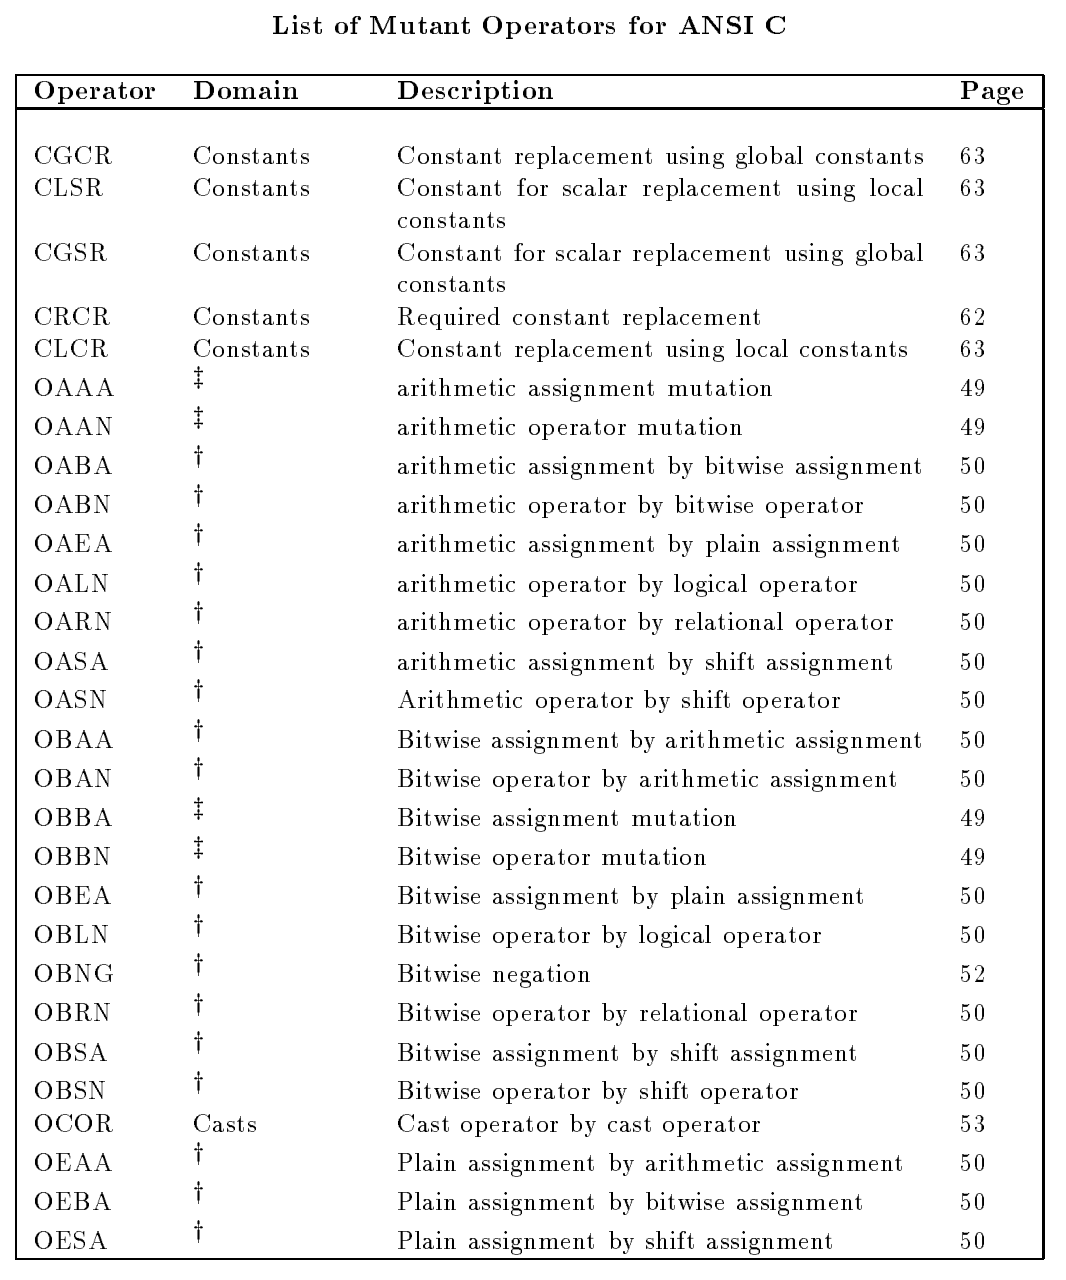
\includegraphics[width=.8\linewidth]{c-operators.png}\par
\par\columnbreak\par
``Each mutant operator belongs to one of the following categories:
1)~statement mutations,
2)~operator mutations,
3)~variable mutations,
and
4)~constant mutations.
''\par
{\scriptsize Source: Hiralal Agrawal et al., \textit{Design of Mutant Operators for the C Programming Language}, Technical Report SERC-TR-41-P, Software Engineering Research Center, Purdue University, 1989\par}
\end{multicols}}

\pitch{\pptQuote{phyllis-frankl.jpg}{Those mutants that compute precisely the same function are called \emph{equivalent} mutants and the others are called \emph{inequivalent} mutants.}{\emph{Phyllis G. Frankl}, Stewart N. Weiss, and Cang Hu, \textit{All-Uses vs Mutation Testing: An Experimental Comparison of Effectiveness?}, Journal of Systems and Software 38(3), 1997}}

\pptBanner{Equivalent Mutants, Example}
\begin{pptWide}{3}
Live Code:\par
{\small\begin{ffcode}
int fibonacci(int n) {
  if (n <= 2) {
    return 1;
  }
  return fibonacci(n - 1)
    + fibonacci(n - 2);
}
\end{ffcode}
}
\par
Tests:\par
{\small\begin{ffcode}
fibonacci(2) == 1;
fibonacci(14) == 377;
\end{ffcode}
}
\par\columnbreak\par
Inequivalent Mutant:\par
{\small\begin{ffcode}
int fibonacci(int n) {
  if (n <= 2) {
    return 1;
  }
  return fibonacci(n (*@\textcolor{red}{\textbf{+}}@*) 1)
    + fibonacci(n - 2);
}
\end{ffcode}
}
\par\columnbreak\par
Equivalent Mutant:\par
{\small\begin{ffcode}
int fibonacci(int n) {
  if (n <= 2) {
    return 1;
  }
  return fibonacci(n - (*@\textcolor{red}{\textbf{2}}@*))
    + fibonacci(n - (*@\textcolor{red}{\textbf{1}}@*));
}
\end{ffcode}
}
\par
\(\uparrow\) You \textbf{can't kill} this one!
\end{pptWide}
\plush{}

\pitch{\begin{multicols}{2}
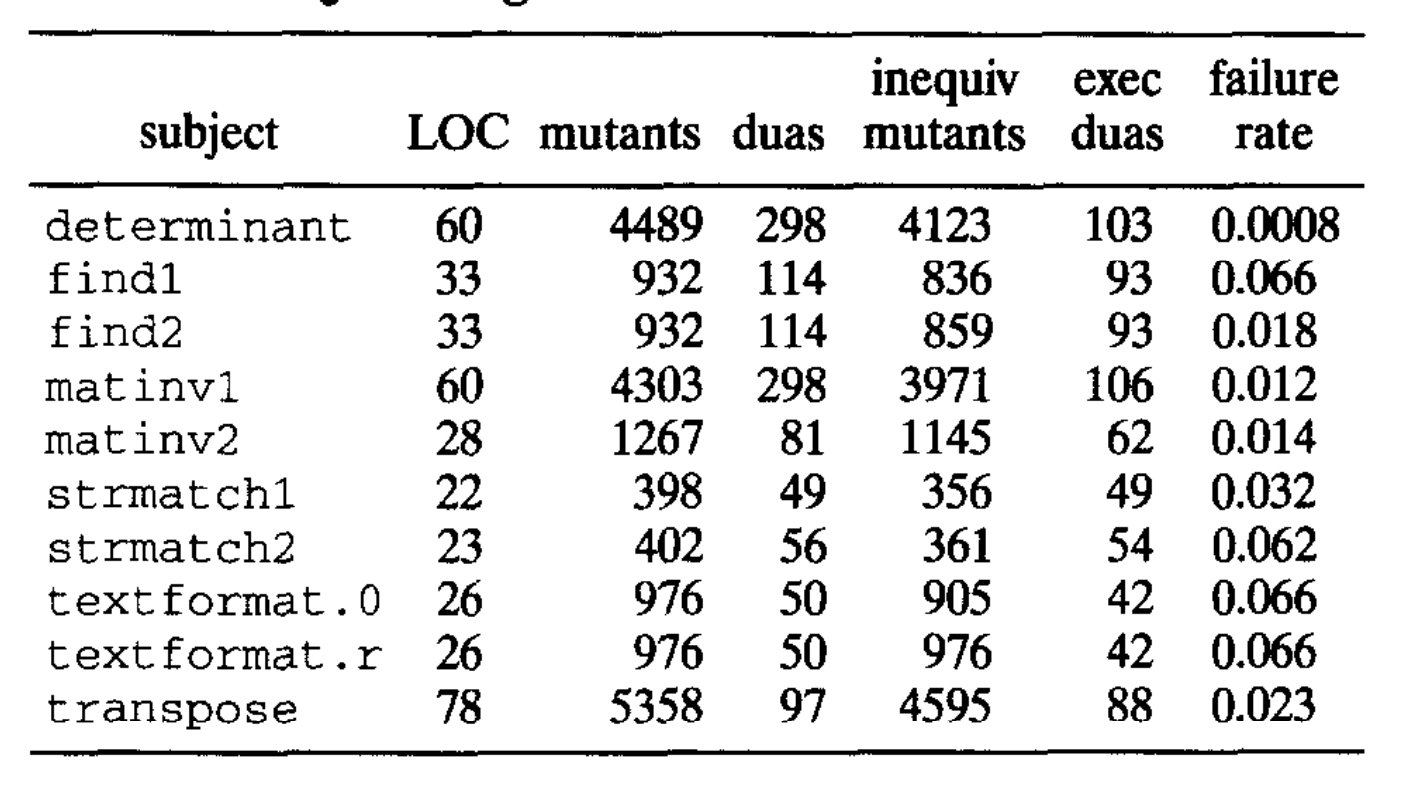
\includegraphics[width=\linewidth]{duas.png}\par
{\scriptsize Source: \emph{Phyllis G. Frankl}, Stewart N. Weiss, and Cang Hu, \textit{All-Uses vs Mutation Testing: An Experimental Comparison of Effectiveness?}, Journal of Systems and Software 38(3), 1997\par}
\par\columnbreak\par
``Mutation coverage is more effective than dua coverage for five subjects, dua coverage --- for two others, and there is no significant difference for the remaining two. \par A definition-use association (\emph{dua} is a triple \(d\), \(u\), \(v\), such that \(d\) is a node in the program's flow graph in which variable \(v\) is defined, \(u\) is a node or edge in which \(v\) is used, and there is a definition-clear path with respect to \(v\) from \(d\) to \(u\).''\par
\end{multicols}}

\pitch{\pptQuote{lionel-briand.jpg}{Our analysis suggests that mutants, when using carefully selected mutation operators and after removing equivalent mutants, can provide a \emph{good indication} of the fault detection \emph{ability} of a test suite.}{James H. Andrews, \emph{Lionel C. Briand} and Yvan Labiche, \textit{Is Mutation an Appropriate Tool for Testing Experiments?}, Proceedings of the 27th International Conference on Software Engineering (ICSE), 2005}}

\pitch{\begin{multicols}{2}
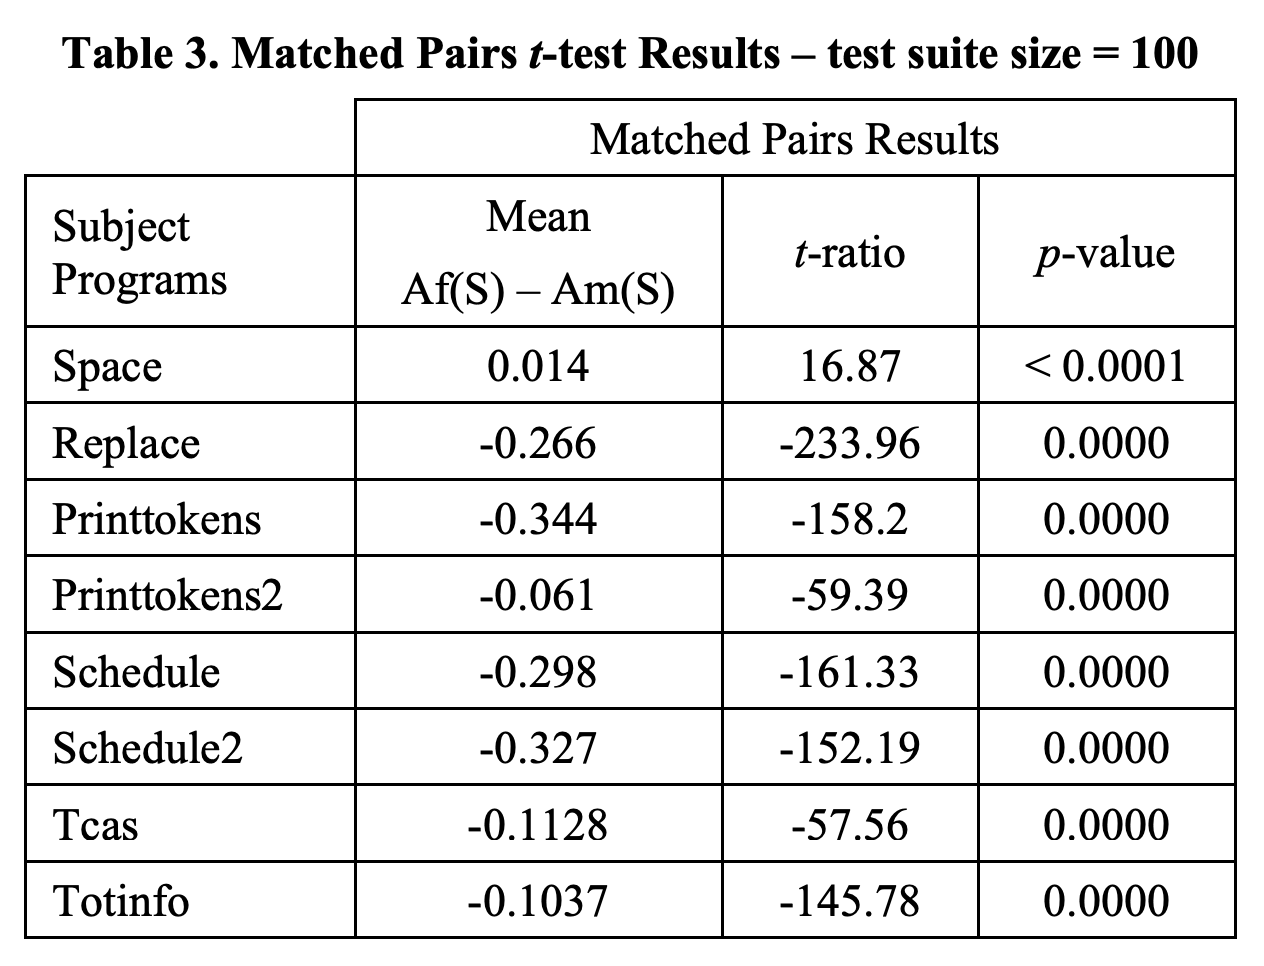
\includegraphics[width=\linewidth]{faults.png}
\par\columnbreak\par
``Average differences range from 6\% to 34\%, with an average of 22\%. \par If one has used mutants to assess a test technique, it will likely look more effective at detecting faults than if one has used the \emph{seeded faults}.''\par
{\scriptsize Source: James H. Andrews, Lionel C. Briand and Yvan Labiche, \textit{Is Mutation an Appropriate Tool for Testing Experiments?}, Proceedings of the 27th International Conference on Software Engineering (ICSE), 2005\par}
\end{multicols}}

\pitch{\pptQuote{yu-seung-ma.jpg}{Comparing with previous mutation systems for procedural programs, \emph{MuJava} is very fast. However, it is relatively slow when it generates and runs lots of mutants.}{\emph{Yu-Seung Ma}, Jeff Offutt, and Yong-Rae Kwon, \textit{MuJava: A Mutation System for Java}, Proceedings of the 28th International Conference on Software Engineering (ICSE), 2006}}

\pitch{\begin{multicols}{2}
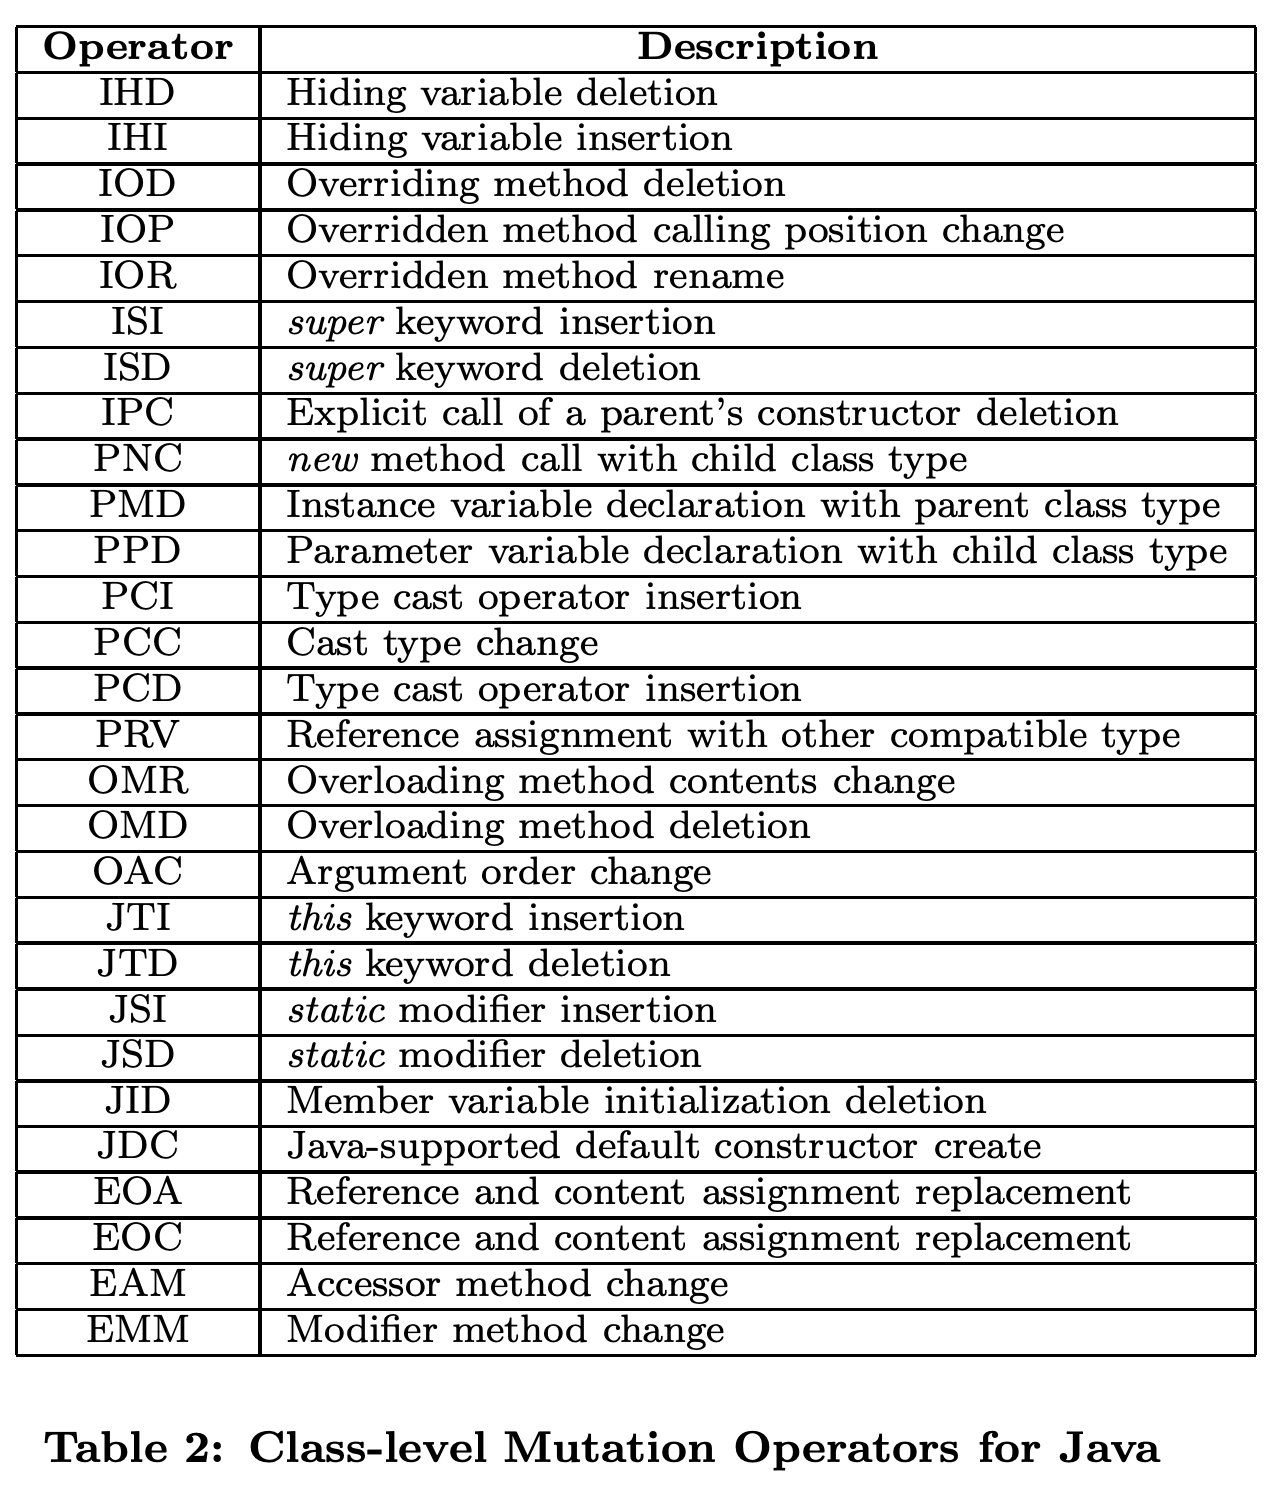
\includegraphics[width=.9\linewidth]{operators.png}
\par\columnbreak\par
``\emph{Method-level} mutation operators handle primitive features of programming languages. They modify expressions by replacing, deleting, and inserting primitive operators. \emph{Class-level} mutation operators handle object-oriented specific features such as inheritance, polymorphism and dynamic binding.''\par
{\scriptsize Source: Yu-Seung Ma, Jeff Offutt, and Yong-Rae Kwon, \textit{MuJava: A Mutation System for Java}, Proceedings of the 28th International Conference on Software Engineering (ICSE), 2006\par}
\end{multicols}}

\pitch{\pptQuote{paul-ammann.jpg}{Three conditions must be present for a failure to be observed:
1)~The location in the program that contains the fault must be reached (\emph{\textbf{R}eachability}).
2)~After executing the location, the state of the program must be incorrect (\textbf{I}nfection).
3)~The infected state must propagate to cause some output of the program to be incorrect (\textbf{P}ropagation).}{\emph{Paul Ammann} and Jeff Offutt, \textit{Introduction to Software Testing}, 2008}}

\pitch{\pptQuote{mark-harman.jpg}{Traditional mutation testing considers only first order mutants, created by the injection of a single fault. Often these first order mutants denote trivial faults that are easily killed. \emph{Higher order mutants} are created by the insertion of two or more faults.}{Yue Jia and \emph{Mark Harman}, \textit{Higher Order Mutation Testing}, Information and Software Technology 51(10), 2009}}

\pitch{\pptQuote{yue-jia.jpg}{One \emph{problem} that prevents mutation testing from becoming a practical testing technique is the \emph{high computational cost} of executing the enormous number of mutants against a test set.}{\emph{Yue Jia} and Mark Harman, \textit{An Analysis and Survey of the Development of Mutation Testing}, IEEE Transactions on Software Engineering 37(5), 2010}}

\pitch{\pptQuote{jie-zhang.jpg}{PMT applies ML to build a predictive model by collecting a series of easy-to-access features (e.g., coverage and mutation operator) on already executed mutants of earlier versions of the project. Based on this model, PMT \emph{predicts} the mutation testing results (i.e., whether each mutant is killed or not) of a new version of project without executing its mutants at all.}{\emph{Jie Zhang}, Ziyi Wang, Lingming Zhang, Dan Hao, Lei Zang, Shiyang Cheng, and Lu Zhang, \textit{Predictive Mutation Testing}, Proceedings of the 25th International Symposium on Software Testing and Analysis, 2016}}

\pitch{Mutation Coverage can be calculated by a few tools:
\begin{itemize}
\item \href{https://pitest.org/}{PIT} for Java
\item \href{https://github.com/stryker-mutator/stryker-js}{StrykerJS} for JavaScript
\item \href{https://github.com/nlohmann/mutate_cpp}{Mutate++} for C++
\item \href{https://github.com/EvanKepner/mutatest}{mutatest} for Python
\item \href{https://github.com/mbj/mutant}{mutant} for Ruby
\end{itemize}}

\end{document}
